
\documentclass[11pt]{article}
% use UTF8 encoding
\usepackage[utf8]{inputenc}
% use KoTeX package for Korean
\usepackage{kotex}
\usepackage{glossaries}
\usepackage{graphicx}
\makeglossaries
\newacronym{cstr}{CSTR}{Continuous Stirred Tank Reactor}
\newacronym{rl}{RL}{Reinforcement Learning}
\newacronym{dqn}{DQN}{Deep Q-Network}
\newacronym{ppo}{PPO}{Proximal Policy Optimization}
\newacronym{ddpg}{DDPG}{Deep Deterministic Policy Gradient}


\usepackage{amsmath}
\begin{document}

\title{가제1:  Nonlinearity를 갖는 CSTR 공정에의 RL 제어 구현 및 성능 개선}
\author{Seunghyun Cho, Hain Lee, Jaehyun Oh}
\date{\today}
\maketitle

 


\section{목표}
본 프로젝트는 Nonlinearity 특성을 지닌 \gls{cstr} 공정에 대하여 강화학습(Reinforcement Learning, RL) 기반 제어 기법을 적용하고, 이를 통해 기존 제어 방법의 한계를 극복하고자 한다.
CSTR 공정은 Nonlinearity 특성을 지님으로써 제어의 어려움을 유발하는 한편, 시스템 제어의 실패가 안전성 문제로 이어질 수 있다. 
따라서 보다 유연하고 적응적인 제어 전략이 요구된다.\\
이에 따라 본 연구에서는 심층 강화학습 알고리즘인 \gls{dqn}, \gls{ppo}, \gls{ddpg} 등을 적용하여 공정의 동적 제어를 수행하고,
\gls{cstr} 공정의 벤치마크인 Van de Vusse 반응을 통해 Reward 함수 설계에 따른 제어 성능 변화 및 공정 안정성 확보 가능성을 검증하고자 한다.


\section{Backgrounds}
\subsection{CSTR}
\gls{cstr}은 화학 공정에서 널리 사용되는 장치로, 반응물의 혼합과 반응을 동시에 수행하는 시스템이다.
이 반응기는 연속적으로 흐르는 유체를 처리하며, 반응의 동적 특성을 고려한 제어가 필요하다. 


\subsection{Process Control}
Process Control은 어쩌구저쩌구 연구분야이다. 이건 어쩌구 저쩌구.


\section{Related Works}

\subsection{Library}
https://github.com/MaximilianB2/pc-gym/tree/main


\subsection{Previous research}
1. 이종민 교수님 연구실 한글논문 \cite{Park2024rl}\\
2. pc gym 논문 \cite{bloor2024pcgym}\\
3. 이종민 교수님 연구실 van de vusse 리뷰논문 \cite{Park2025pc} \\
4. 벤치마크로써 CSTR nonlinearity 다룬 논문 \cite{chen1995benchmark} \\
5. PPO 활용한 논문 \cite{Yu2025ppo}

\section{계획}
1. State, Action value 정의(반응을 좀 더 복잡하게-이종민교수님 한글논문에 있는 식 또는, tank level 추가하기-이건 PPO 논문에서 다뤘음)\\
\begin{figure}[h!]
    \centering
    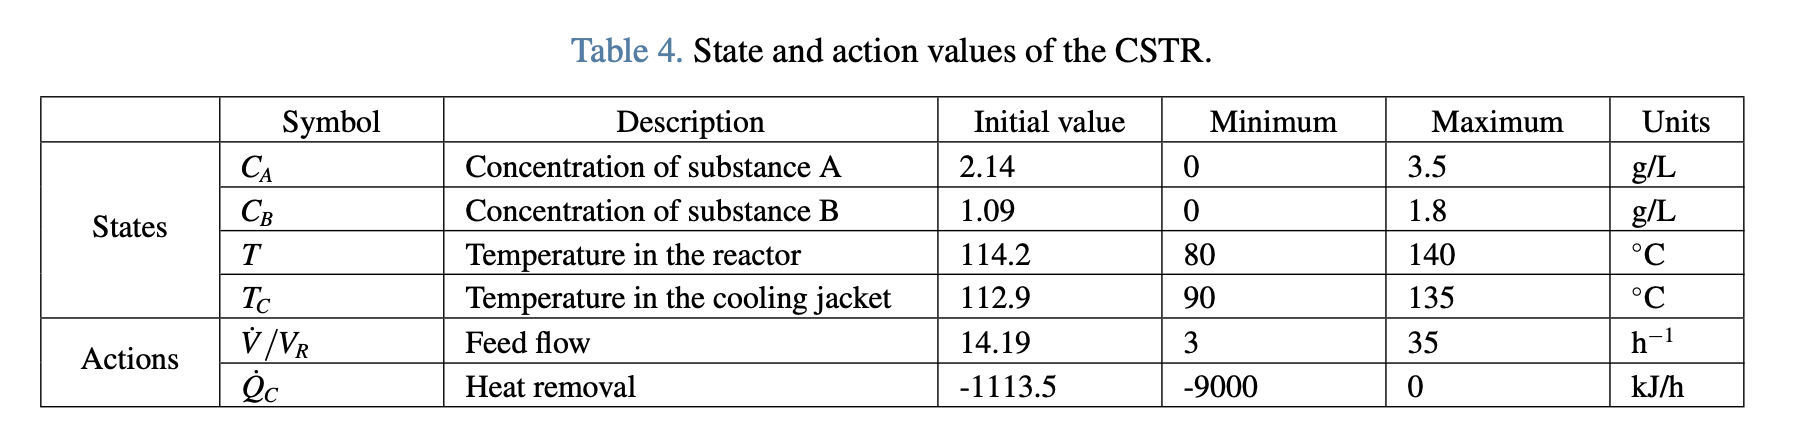
\includegraphics[width=\textwidth]{ref_table1.png} % 또는 .png, .pdf 등
    \caption{Defined states and actions in previous research}
    \label{fig1}
\end{figure}
\\
2. 코드 CSTR 수정 
+ 반응은 벤치마크중 하나인 Van de vusse(강화학습 기반 화학 공정 제어 성능 향상을 위한 보상 함수 시뮬레이션 연구 - 식9)
위 논문의 식에 맞게 소스코드 수정해야함\\
3. DQN, PPO, (DDPG) 를 활용하여 ㅡㅡㅡ. \\
4. 리워드 함수에 따른 공정 제어 성능 확인(이건 미정이지만 할 수 있을듯)\\


\bibliography{references}



\end{document}

